\part{Misura della $\lambda$ della riga gialla del sodio}
\section{Scopo e strumentazione}
	In questa parte dell'esperienza si è determinata la lunghezza d’onda $\lambda_{\text{Na}}$ della riga spettrale emessa da una lampada al sodio.

	La strumentazione impiegata in questa prima parte si compone di:
	\begin{itemize}
		\item uno spettroscopio a	prisma, schematicamente rappresentato in \figurename{ \ref{fig:prisma}} dalla risoluzione teorica di $1/60$ di grado;
		\item una lampada al cadmio, utilizzata in fase di calibrazione del quale si assume di conoscere la lunghezza d'onda delle righe spettrali.
		\item una lampada al sodio.
	\end{itemize}

	\begin{figure} [H]
		\centering
		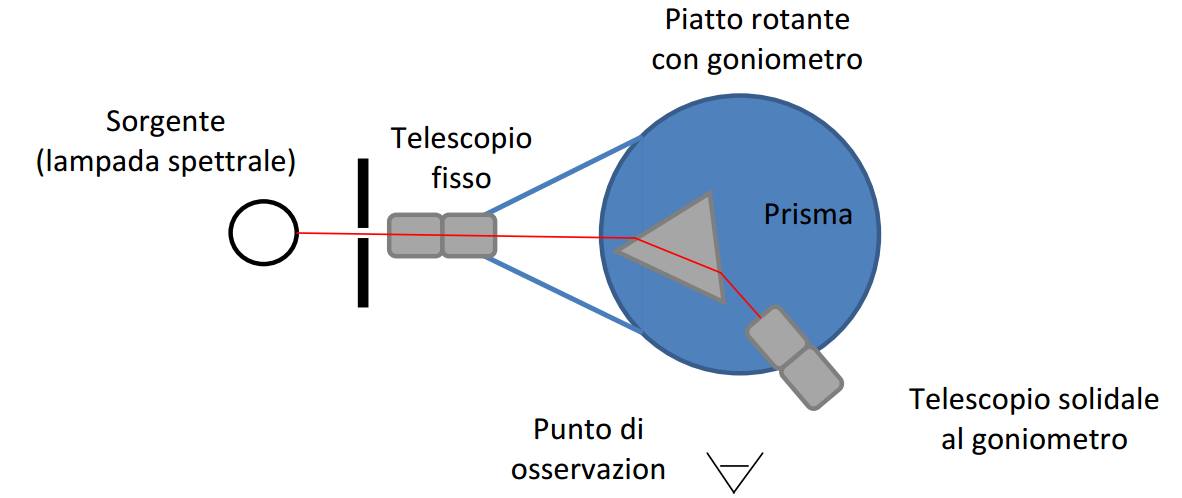
\includegraphics[width=0.9\textwidth]{../Figs-tabs/prisma}
		\caption{Schema dell'apparato impiegato.}
		\label{fig:prisma}
	\end{figure}
